\chapter{INTRODUCTION}
\thispagestyle{plain}

\label{Introduction}

In this chapter we briefly describe the android platform and the current threat landscape in mobile devices domain. Next, we discuss the motivation for our work, the problem this thesis tries to solve, and describe the proposed solution. Chapter two briefly touches upon prior work in this domain. Chapter three describes the design and architecture of the proposed malwares detection system while giving a walkthrough of the multiple modules in system and their individual role. Chapter four dives into the methodology we followed while conducting our experiments and how we tested its effectiveness. Chapter five describes the results obtained from our experiments followed by a short concluding piece which describes possible enhancements and future work.

\section{Android Platform}

In the last few years smartphone usage has increased dramatically. It is estimated that in year 2014 USA would have 163.9 million~\cite{26} smartphone users and globally there would 1.204 billion~\cite{27} users. 
\begin{figure}[htp]
\centering
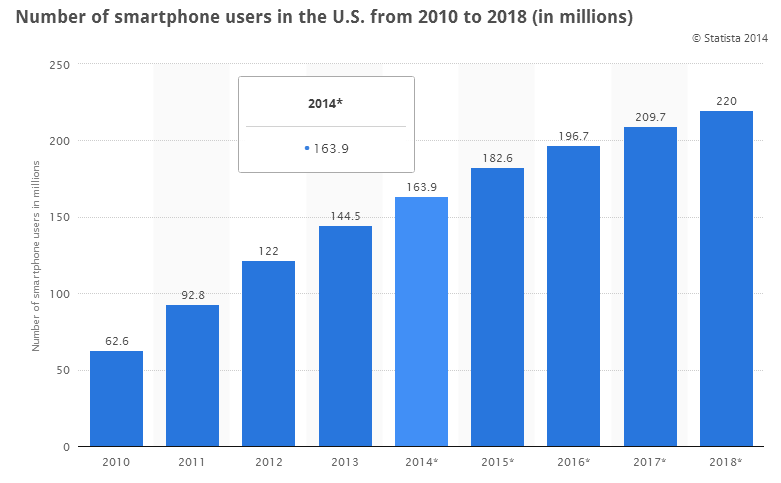
\includegraphics[width=\textwidth, height=\textheight, keepaspectratio]{1_SmartPhoneUsage}
\caption{Smartphone Usage in USA}
\label{fig:1_SmartPhoneUsage}
\quad
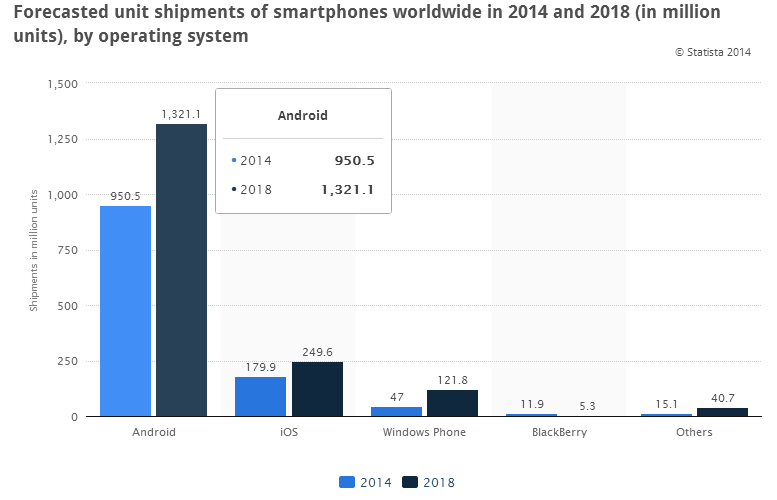
\includegraphics[width=\textwidth, height=\textheight, keepaspectratio]{2_MarketShareByOS}
\caption{Android OS Market Share 2014 - 2018}
\label{fig:2_MarketShareByOS}
\end{figure}

Figure \ref{fig:1_SmartPhoneUsage} provides current smartphone usage trends in USA. Smartphone technology is advancing over period of time providing higher computational power, newer sensors, improved network speed and with higher battery capacity. Due to this  smartphones are making inroads to newer and wider application areas, e.g education, retail, hospitality, insurance, entertainment and many more. 

Android is most popular operating system world wide and it is expected to be shipped on 1.32 billion~\cite{27} smartphones in year 2018. This kind of popularity not only attracts the attention of developers but also from those with malicious intentions. Android applications can be downloaded from various market places. Usually developer needs to cryptographically sign the application before publishing it on the android store, but most developers use self-signed certificates for this purpose. Due to this practice there exists limited authentication mechanism. Also there are tools~\cite{28} to reverse engineer and repackage these applications with custom code inserted in to it. As a result, repackaged application is most used attack vector on android platform. 

The rapid increase in the amount of new repackaged malicious applications is of great concern, since many of the modern antivirus products are not able to keep up with this growing threat and keep their malware signature database up to date. A research study by F-Secure Labs~\cite{29} shows that less than 5\% of all recorded malware specimens were detected by existent malware scanners.

The detection rate is even worse when code obfuscating techniques are used while repackaging these applications. The malicious payload can be modified in multiple different ways to evade the signature based antivirus. For example inserting junk code that doesn't alter functionality, by rearranging the code structure and by replacing part of code with equivalent code. 

These kind of changes allow repackaged applications to produce various variants of similar application with different signatures. Though the signature is different, in general the behaviour of the application remains same. Due to this, it is impossible to detect all variants of malware with a few known signatures. This problem can be addressed by dynamically analysing behaviour of application and its interaction with android platform. Here we model the behaviour of application by analysing the system call sequence and its distribution. 

This thesis aims at finding robust and effective techniques for detection and classification of android malware. Though malware detection is primary focus of this thesis work, we also want to classify the given malware to its known family. As android malware families are well documented for their infection mechanism, behaviors and possible removal steps, knowing malware family name provides valuable information. This information would be useful for narrowing the scope of the investigation and reduce the response time required to mitigate the attack. We use android system calls as feature set for building different classifiers. Classifiers are built using boosting on an ensemble of weak learners. We conduct an extensive experimental study to evaluate the performance of different boosting techniques and ensembles. The classification done using syscalls distribution is much robust and shows significant association with the malware's family. For detection purpose we also build deeplearning model, using Stacked Denoising Autoencoder (SdA) approach. The SdA model is most robust with lowest false positive rate.

While constructing features for malware detection and classification we perform dynamic analysis of each specimen app on an instrumented android device. Each application run provides log files with system call sequence that was observed by android platform for given application. We build the system call distribution using these log files and use that as a feature set for classifying given application to malicious or benign app. Also we use this distribution for classifying the given dataset of malicious apps into corresponding known malware families.

Before performing this analysis, caution should be taken as these malicious apps are variants of repacked applications. For collecting reasonable system calls multiple runs needs to be done. Also for avoiding any bias towards specific system calls we normalize the dataset using Z-score. Our experiments show that malware detection using SdA classifier provides better performance and accuracy than other approaches that we evaluated. Several experiments were performed to check for the robustness and the validity of the claim that SdA performs better with highest detection rate and lowest false positive rate. The stability of SdA is tested by introducing noise in the input data set.